\documentclass[pdftex,12pt,a4paper]{article}

\usepackage[pdftex]{graphicx}
\usepackage{graphicx}
\usepackage{picture}
\usepackage{graphics}
\usepackage{amsmath} % for argmax
\usepackage{bm} % used for bolding the equation

\newcommand{\HRule}{\rule{\linewidth}{0.5mm}}
\DeclareMathOperator*{\argmin}{argmin}

\begin{document}

\begin{titlepage}

\begin{center}


% Upper part of the page

\includegraphics[width=0.15\textwidth]{./uml_logo}\\[5cm]    

\textsc{\LARGE Computer Graphics I}\\[1.5cm]

\textsc{\Large Literature Reivew II}\\[0.5cm]


% Title
\HRule \\[0.4cm]
{ \huge \bfseries Image Annotation Techniques}\\[0.4cm]

\HRule \\[1.5cm]

% Author and supervisor
\begin{minipage}{0.4\textwidth}
\begin{flushleft} \large
\emph{Author:}\\
Chang \textsc{Liu}
\end{flushleft}
\end{minipage}
\begin{minipage}{0.4\textwidth}
\begin{flushright} \large
\emph{Teacher:} \\
Dr.~Haim \textsc{Levkowitz}
\end{flushright}
\end{minipage}

\vfill

% Bottom of the page
{\large \today}

\end{center}

\end{titlepage}

\section{Overview}

In this section, I'm going to present two papers that talks about the image annotation. As we
all know that image annotation is becoming very popular nowadays, but automatic image annotation methods based on searching for correlations require a quality training image dataset. 

For a target image, its annotation is predicted based on a mutual similarity of the target image to the training images. One of the main problems of current methods is their low effectiveness and scalability if a relatively large-scale training dataset is used.

So starting from this point, I'm going to do some paper reading and research on this topic and gives two seperated
description about their techniques of image annotation.

\section{Image Annotation}
In this section, I'm going to talk about the technique that is used in the first paper \textbf{"ANNOR: Efficient image annotation based on combining local and global features"}, this paper is selected from Computers \& Graphics, 2015. The main idea of this paper is a new approach named
“Automatic image aNNOtation Retriever” (ANNOR) for acquiring annotations for target images, which is
based on a combination of local and global features. According to their report, the approach gives a very good and precise result for image annotation.

\section{ANNOR}
Focusing on visual query forms, many content-based image retrieval methods and techniques have been proposed,
but they have several limitations. On one hand, in query-by-example-based
methods a query image is often absent. On the other hand, query by-sketch
approaches are too complex for common users and
a visual content interpretation of a user image concept is difficult.

Facing such a broad challenge and research focus, automatic image annotation is becoming the frontier of 
different fields such as image analysis, machine learning and information retrieval. In
present, to create a general system for automatic image annotation
based on object recognition is practically impossible. Even though many approaches have been proposed, there
have been very few breakthrough in these fields.

After carefully analyzing the problem's source, a new approach ANNOR is proposed to solve it.
ANNOR is short for the "Automatic image aNNOtation Retriever", which is retrieve the image by combining the global
and local features.

For a problem, there have been some problems that must be solved:

1) Which image representation is appropriate to describe image?
The objects in images are often occluded and appear in poor
lighting and exposure.

2) Which image features can be extracted to describe or characterize
the visual content? A feature is represented by a numerical
feature vector (descriptor), by which we are able to describe a
part of image content. In general, there are three essential
requirements for the descriptors, their degree of robustness,
discrimination ability and efficiency. The robustness represents
invariance to the geometrical changes (e.g., viewpoint, zoom,
object orientation) and noise-like signal distortions. The discrimination
maximizes difference among non-duplicates and
minimizes difference among duplicates. The feature extraction
and matching requires fast computation.

3) How much is the spatial and time complexity (computational cost) for a new method

In the paper the author proposes a method for automatic image annotation
using relatively large-scale image “training” dataset. By combining local
and global features to ensure robustness and generalization needed by
complex queries, they focus more on performance and scalability.
For indexing and clustering features, they use disk-based locality
sensitive hashing. To obtain annotation for a given target image, the
approach is based on the way how people manually annotate images.


\section{Contribution}
For this paper the most important contribution is that it gives us the key point that combines the global
and local features together, by calculating the keyword of each image using these feature, we could get the
most potential annotated keyword.

\section{Comparable paper}
For the second paper, I'm going to talk about the content of \textbf{"An evaluation of descriptors for large-scale image retrieval from sketched feature lines"}, this paper gives another view about the image retrieval method. Different from
previous one, this paper mainly talks about the details about image retrieval towards a large-scale database.From the first
page we know that a large-scale database could lead to a lot of technical problem when doing the image annotations, in this
paper, however, we could know that for a large-scale dataset, it is also challenging to get a very efficient descriptor. In
this paper, the author presents a system for a sketch-based image retrieval that yield interactive search results on a database of more than one million images By using both the ARP and EHD descriptor as a baseline for evaluation and comparing
their performance to that of the Tensor and HOG descriptor, it shows that Tensor and HOG descriptor efficiently capture distribution of location and orientation of gradients in the images but differ in the way this information is encoded.

\section{Descriptor}
In the second paper, the author uses two descriptor that shows very effective in their paper, which is Tensor and EHD descriptor. In this section I will talk more about these two descriptors as they're used successfully in the first paper and
shows a wide potential in future research.
\subsection{EHD}
EHD is the short form of \textbf{"edge histogram descriptor"}, it is proposed in MPEG-7 standard for texture image characterization, the following figure shows the EHD's function for distinguishing five types of edges:

\begin{center} % add this to make the figure shows in the middle of the pages
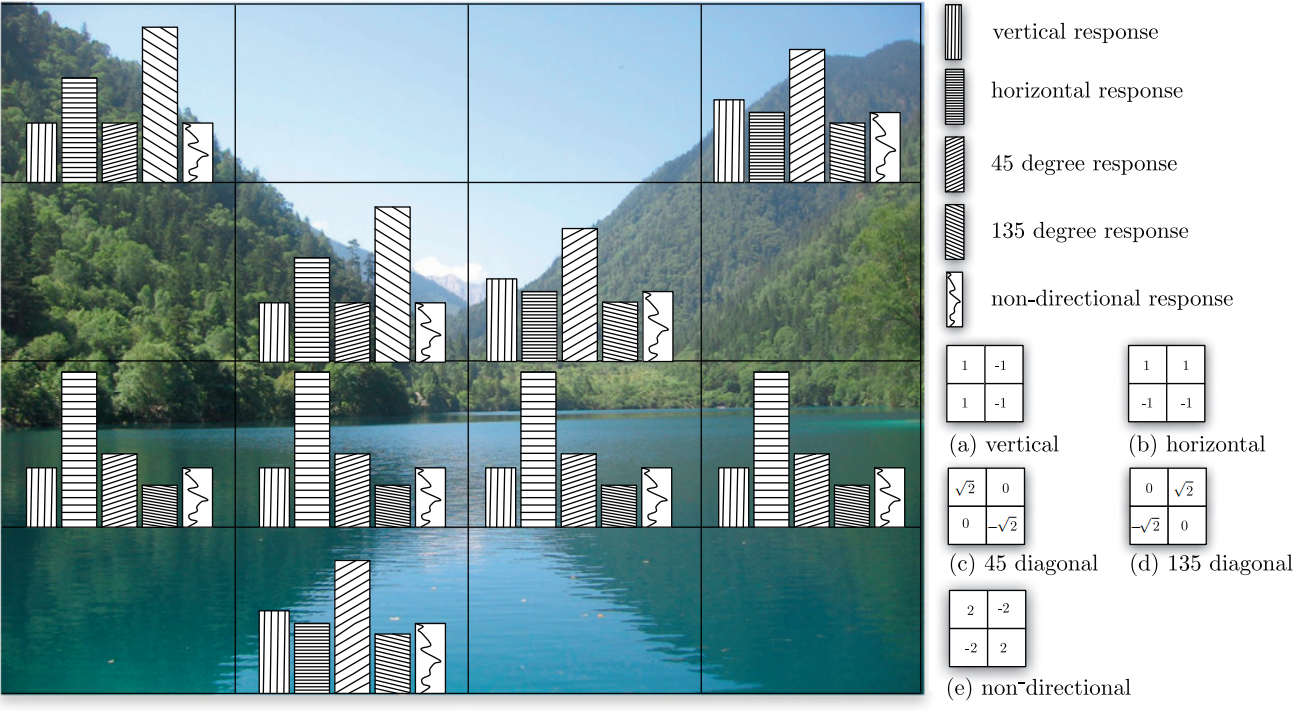
\includegraphics[width=4.00in,height=2.00in]{let-rev2_1.png}
%\caption{EHD descriptor for distinguishing the image}
\end{center}

The EHD represents the distribution of five types of edges in
local image patches. As illustrated in the above figure, the image is subdivided
into $k \times k$ non-overlapping cells. The edge distribution in each cell
is characterized by a 5-bin histogram, distinguishing five different
types of edges: vertical, horizontal, $45^{\circ}$, $135^{\circ}$ and non-directional edges. 
A histogram is computed for each of the cells individually, resulting in a feature vector of size 5$k^{2}$.


\section{Tensor Descriptor}
The tensor descriptor is the system matrix which maximize the single vector's distance between the scalar image and the original image.
Let \textbf{x} be a unit vector, which we want to define such that it represents the main direction in cell $C_{ij}$.
As $\bm{x^{T}g_{uv}}$ attains a maximum if $\bm{x||g_{uv}}$ we pose the definition of \textbf{x} as the following optimization

\begin{displaymath}{x}=\arg\underset{x\in\mathcal{X}}{\min}\,{\sum_{i=1}^{n}}(x^{T}g_{uv})
\end{displaymath}

In order to detect similarly oriented image edges independently of the magnitude of the edges, we store the structure
tensor normalized by its Frobenius norm, so that this descriptor has a tense representation of image's texture.


\section{summary}
From the above section, I know that these papers have made a wide research on the topic of image annotation and feature
descriptors. I select two of them because the first contains the annotation technique that interests me so much, the second
one is chosen because they share the same descriptor that could enhance the representation of image, and it is credential for
image annotations.

According to current research, image features and descriptors are two factors that are very important in today's image and
graphic research. We all know that different features and descriptors could have great impact on the precision, so both the
first and second paper gives the evaluation on the process, while the first one focus on combining the global feature and local feature together to achieve a good performance, the second one focus on selecting a better descriptors for image retrieval in a large dataset. Both of them have done great job in making the image processing jobs more efficient and precise. After reading these two papers, I have got to know better about how to improve the precision and efficiency for
the images, and it's really a lot of help for me to the this kind of research.




\end{document}